\documentclass[]{article}

\usepackage[numbers]{natbib}
%\usepackage[authoryear,round,longnamesfirst,numbers]{natbib}
\usepackage{fullpage}
\usepackage{amsmath,amssymb,amsthm}
\usepackage{tikz}
\usepackage{pgfplots}
\usepackage{booktabs}
\usepackage{units}
\usepackage{subfig}
\usepackage{verbatim}

\usepackage{algorithm}
\usepackage{algpseudocode}



\newcommand{\Mat}[1]{\mathsf{#1}}  %% matrices
\newcommand{\op}[1]{\mathcal{#1}}  %% operators
\newcommand{\flop}{\operatorname{flop}}


\theoremstyle{plain}
%\theoremstyle{remark}
%\theoremstyle{definition}
\newtheorem{example}{Example}
\newtheorem{definition}{Definition}
\newtheorem*{note}{Note}
\newtheorem*{remark}{Remark}


\begin{document}

\title{Kernels of the black-box FMM}
\author{Matthias Messner}
%\date{\today}
\date{February 28, 2013}
\maketitle

\begin{abstract}
  This document explains in detail the (CPU) kernels of the black-box FMM we
  use and points out differences to the paper by~\citet{fong09a}. 
\end{abstract}

\tableofcontents



\section{Basics}
\label{sec:basics}

We compute the interaction between two cells $X,Y\subset\mathbb{R}$. The cell
$Y$ contains all source particles $\{y_j\}_{j=1}^N$ and the cell $X$ contains
all target particles $\{x_i\}_{i=1}^M$. The goal is to compute the
interactions efficiently by exploiting the Chebyshev interpolation scheme
\begin{align}
  \label{eq:fast_summation}
  f_i &= \sum_{j=1}^N K(x_i,y_j)w_j \quad \text{for } i=1,\dots,M \nonumber \\
  &\sim \sum_{m=1}^\ell S_\ell(x_i,\bar x_m) \sum_{n=1}^\ell K(\bar
  x_m, \bar y_n) \sum_{j=1}^N S_\ell(y_j,\bar y_n) w_j
\end{align}
with the interpolation points $\bar x\in X$, respectively $\bar y\in Y$. The
interpolation polynomial is defined as
\begin{equation}
  \label{eq:interpolation_polynomial}
  S_\ell(x, \bar x_m) = \frac{1}{\ell} + \frac{2}{\ell} \sum_{i=1}^{\ell-1}
   T_i(x) \, T_i(\bar x_m).
\end{equation}
The individual FMM kernels can be identified in Eqn.~\eqref{eq:fast_summation}
as
\begin{itemize}
\item P2M (particle-to-moment) at the leaf-level and M2M (moment-to-moment) at
  all other levels:
  \begin{equation}
    \label{eq:m2m}
    W_n = \sum_{j=1}^{N} S_\ell(y_j,\bar y_n) w_j \quad \text{for }
    n=1,\dots,\ell
  \end{equation}
\item M2L (moment-to-local):
  \begin{equation}
    \label{eq:m2l}
    F_m = \sum_{n=1}^\ell K(\bar x_m, \bar y_n) W_n \quad \text{for }
    m=1,\dots\ell
  \end{equation}
\item and L2P (local-to-particle) at the leaf-level and L2L (local-to-local)
  at all other levels:
  \begin{equation}
    \label{eq:l2l}
    f_i \sim \sum_{m=1}^\ell S_\ell(x_i,\bar x_m) F_m \quad \text{for }
    i=1,\dots,M.
  \end{equation}
\end{itemize}
For the sake of readability we omit the mapping from and to the reference
interval $[-1,1]$. Moreover, the extension of the interpolation scheme in
$\mathbb{R}$ to the tensor-interpolation in $\mathbb{R}^3$ is going to be
explained in detail in Sec.~\ref{sec:tensorinterpol}.

\section{M2L --- optimization based on symmetries}
\label{sec:m2l}
In this section we consider the M2L kernel. In Eqn.~\eqref{eq:m2l} it is
presented for the one-dimensional case. Its extension to the three-dimensional
case is less involving then for the other kernels. We have the cells
$X,Y\subset\mathbb{R}^3$ and the M2L kernel reads in $\mathbb{R}^3$ as
\begin{equation}
  \label{eq:m2l_3d}
  F_m = \sum_{n=1}^{\ell^3} K(\bar x_m, \bar y_n) W_n \quad \text{for }
  m=1,\dots\ell^3.
\end{equation}
In the following we introduce an improved version of the M2L kernel for the
black-box FMM which is favorable over the approach presented in
\citep{fong09a} in terms of precomputation time, number of required floating
point operations \unit{(flops)} and cache reuse. First, we show the advantage
of individual SVDs, second, we exploit symmetries in the arrangement of the
far-field interactions and, finally, the combination of both approaches leads
to the new M2L kernel.

\paragraph{Far-field interactions} Normally, in $\mathbb{R}^3$ the far-field
is limited to the at most $26$ near-field interactions of the
parent-cell. This leads to at most $189$ far-field interactions
$I_Y=\{Y_s:1\le s\le 189\}$ (source cells) for each target cell $X$. Most
kernel functions are homogeneous (if we scale the distance between source $y$
and target $x$ by a factor of $\alpha$ the resulting potential is scaled by
$\alpha^n$, where $n$ is a constant and depends on the kernel
function). Hence, the M2L kernels of all $316$ possible far-field interactions
for all cells need to be computed only once. In order to identify the
far-field interactions we introduce translation vectors $t = (t_1,t_2,t_3)$
which give the relative position of a cell-pair $(X,Y)$. All its components
are limited to the interval $t_i\in[-3,3]$ (near-field interactions of
parent-cell) and $|t|>\sqrt{3}$ (excludes near-field interactions) must be
true. This leads to $7^3-3^3=316$ different translation vectors.

\begin{note}
  If we use kernel functions which are not homogeneous, such as the
  Lenard-Jones potential $K_{LJ}(r) = \frac{1}{r^{12}} - \frac{1}{r^6}$ the
  only difference is that we cannot compute the M2L kernels all far-field
  interactions only in the reference cells (all dimensions are in $[-1,1]$)
  and scale them on different levels but we have to compute them on each
  level. This affects the precomputational time and the memory requirement
  (both $h-2$ times as large as the one for the homogeneous case).
\end{note}

\subsection{Individual SVDs}
\label{sec:16svds}
We apply individual SVDs to each of the $316$ far-field interactions and
compare the resulting cost to the approach proposed in \citep{fong09a} in
Tab.~\ref{tab:cost_of_one_vs_many_svds}.
\begin{table}[htbp]
  \caption{Comparison of both M2L optimizations}
  \label{tab:cost_of_one_vs_many_svds}
  \centering
    \begin{tabular}{c | c c | c}
      \toprule
      $Acc$ & $r_{\text{big}}$ & $r_{\text{ave}}$ &
      cost$_{\text{ave}}/$cost$_{\text{big}}$ \\  
      \midrule
      3 &  19 & 4.6  & 0.69 \\
      5 &  67 & 11.2 & 0.62 \\
      7 & 150 & 22.2 & 0.67 \\
      \bottomrule
  \end{tabular}
\end{table}
The first column gives the accuracy defined as
$(\ell,\varepsilon_{\text{SVD}})=(Acc,10^{-Acc})$ and the second and third
column compare the low-rank $r_{\text{big}}$ to $r_{\text{ave}}$ (the average
low-rank of all $316$ far-field interactions in our approach).  Finally,
column four shows the ratio of the computational costs of applying them, they
are defined as $\text{cost}_{\text{big}} = \mathcal{O}(316 \cdot
r_{\text{big}}^2)$ and $\text{cost}_{\text{ave}} = \mathcal{O}(316 \cdot
2\ell^3r_{\text{ave}})$. Where do these numbers come from? \citet{fong09a}
write the $t=1,\dots,316$ far-field interactions as
$\Mat{K}_t\sim\Mat{UC}_t\Mat{V}^\top$, hence, the M2L kernel consists in $316$
matrix-vector products with $\Mat{C}_t\in\mathbb{R}^{r_{\text{big}}\times
  r_{\text{big}}}$. We represent the far-field interactions as
$\Mat{K}_t\sim\Mat{U}_t\Mat{\Sigma}_t\Mat{V}_t^\top$ with the matrices
$\Mat{U}_t,\Mat{V}_t\in\mathbb{R}^{\ell^3\times r_{\text{t}}}$. Note that the
average rank is defined as $r_{\text{ave}} =
\nicefrac{\left(\sum_{t=1}^{316}r_t\right)}{316}$.

\subsection{Symmetries}
\label{sec:symmetries}

Evidently, there are symmetries in the arrangement of the far-field
interactions. By exploiting them, the $316$ interactions can be reduced to
$16$ only. How do we do that?  First, by considering symmetries given by the
axial planes, we obtain $8$ octants as shown in
Fig.~\ref{fig:interaction_box}. We use the octant with $i,j,k\ge 0$ as
reference octant. In this way we reduce the $316$ interactions to only
$4^3-2^3=56$ different interactions.
\begin{figure}[htbp]
  \centering
  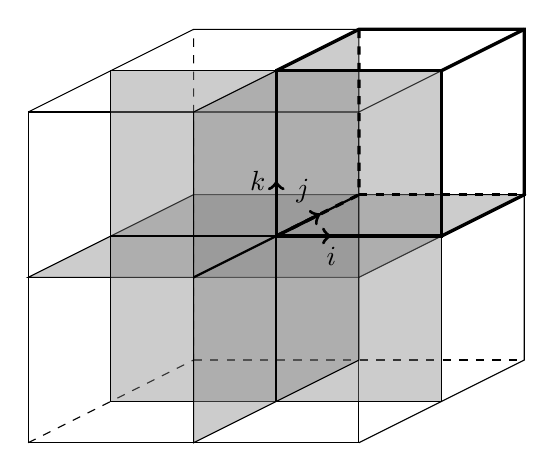
\begin{tikzpicture}[scale=.7]
    \draw (-3,-3) -- (3,-3) -- (3,3) -- (-3,3) -- cycle;
    \draw (3,-3) -- (6,-1.5) -- (6,4.5) -- (0,4.5) -- (-3,3);
    \draw (3,3) -- (6,4.5);
    \draw[dashed] (-3,-3) -- (0,-1.5) -- (0,4.5);
    \draw[dashed] (0,-1.5) -- (6,-1.5);

    \filldraw[thin,fill=gray, fill opacity=.4]
    (-3,0) -- (3,0) -- (6,1.5) -- (0,1.5) -- cycle;
    \filldraw[thin,fill=gray, fill opacity=.4]
    (-1.5,-2.25) -- (4.5,-2.25) -- (4.5,3.75) -- (-1.5,3.75) --cycle;
    \filldraw[thin,fill=gray, fill opacity=.4]
    (0,-3) -- (3,-1.5) -- (3,4.5) -- (0,3) -- cycle;

    \draw[thick] (-1.5,.75) -- (4.5,.75);
    \draw[thick] (1.5,-2.25) -- (1.5,3.75);
    \draw[thick] (0,0) -- (3,1.5);

    \draw[very thick,->] (1.5,.75) -- (2.5,.75) node[below]{$i$};
    \draw[very thick,->] (1.5,.75) -- (2.3,1.15) node[above left]{$j$};
    \draw[very thick,->] (1.5,.75) -- (1.5,1.75) node[left]{$k$};

    \draw[very thick]
    (1.5,.75) -- (4.5,.75) -- (4.5,3.75) -- (1.5,3.75) -- cycle;
    \draw[very thick]
    (4.5,.75) -- (6,1.5) -- (6,4.5) -- (3,4.5) -- (1.5,3.75);
    \draw[very thick] (4.5,3.75) -- (6,4.5);
    \draw[very thick,dashed] (1.5,.75) -- (3,1.5) -- (3,4.5);
    \draw[very thick,dashed] (3,1.5) -- (6,1.5);
  \end{tikzpicture}
  \caption{Box of size $7\times 7\times 7$ showing the reference octant with
    $i,j,k\ge 0$ (contains $4^3-2^3=56$ far-field interactions).}
  \label{fig:interaction_box}
\end{figure}
Next, we exploit symmetries given by diagonal planes, $i=j$ in
Fig.~\ref{fig:ji}, $i=k$ in Fig.~\ref{fig:ki} and $j=k$ in
Fig.~\ref{fig:kj}.
\begin{figure}[htbp]
  \centering
  \subfloat[$j\le i$]{
    \label{fig:ji}
    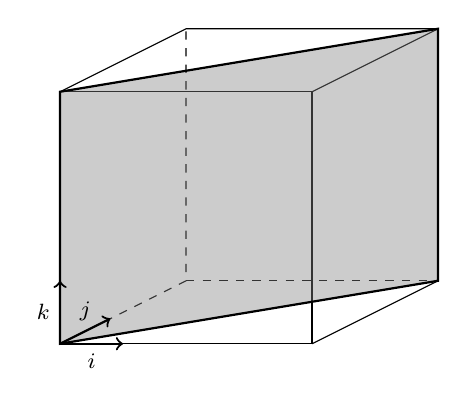
\begin{tikzpicture}[scale=.8,font=\footnotesize]
      \draw (0,0) -- (4,0) -- (4,4) -- (0,4) -- cycle;
      \draw (4,0) -- (6,1) -- (6,5) -- (2,5) -- (0,4);
      \draw (4,4) -- (6,5);
      \draw[dashed] (0,0) -- (2,1) -- (2,5);
      \draw[dashed] (2,1) -- (6,1);
      \filldraw[thick, fill=gray, fill opacity=.4]
      (0,0) -- (6,1) -- (6,5) -- (0,4) -- cycle;
      \draw[thick,->] (0,0) to node[below]{$i$} (1,0);
      \draw[thick,->] (0,0) to node[above]{$j$} (.8,.4);
      \draw[thick,->] (0,0) to node[left]{$k$} (0,1);
    \end{tikzpicture}
  }
  \hfill
  \subfloat[$k\le i$]{
    \label{fig:ki}
    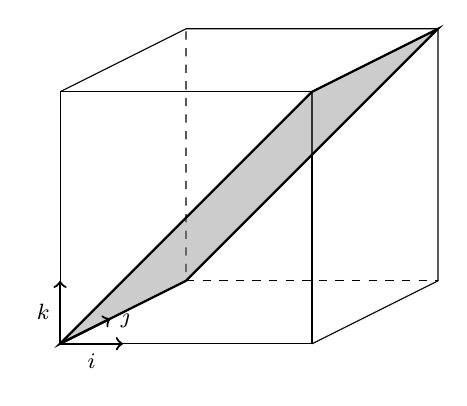
\begin{tikzpicture}[scale=.8,font=\footnotesize]
      \draw (0,0) -- (4,0) -- (4,4) -- (0,4) -- cycle;
      \draw (4,0) -- (6,1) -- (6,5) -- (2,5) -- (0,4);
      \draw (4,4) -- (6,5);
      \draw[dashed] (0,0) -- (2,1) -- (2,5);
      \draw[dashed] (2,1) -- (6,1);
      \filldraw[thick, fill=gray, fill opacity=.4]
      (0,0) -- (4,4) -- (6,5) -- (2,1) -- cycle;
      \draw[thick,->] (0,0) to node[below]{$i$} (1,0);
      \draw[thick,->] (0,0) -- (.8,.4) node[right]{$j$};
      \draw[thick,->] (0,0) to node[left]{$k$} (0,1);
    \end{tikzpicture}
  }
  \hfill
  \subfloat[$k\le j$]{
    \label{fig:kj}
    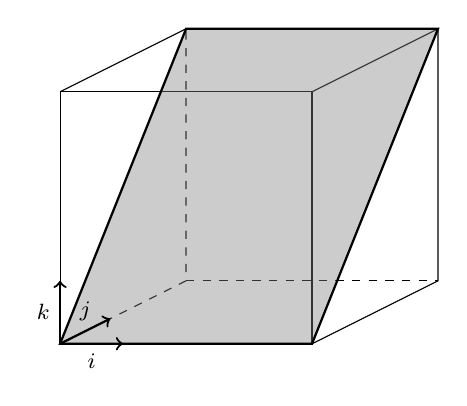
\begin{tikzpicture}[scale=.8,font=\footnotesize]
      \draw (0,0) -- (4,0) -- (4,4) -- (0,4) -- cycle;
      \draw (4,0) -- (6,1) -- (6,5) -- (2,5) -- (0,4);
      \draw (4,4) -- (6,5);
      \draw[dashed] (0,0) -- (2,1) -- (2,5);
      \draw[dashed] (2,1) -- (6,1);
      \filldraw[thick, fill=gray, fill opacity=.4]
      (0,0) -- (4,0) -- (6,5) -- (2,5) -- cycle;
      \draw[thick,->] (0,0) to node[below]{$i$} (1,0);
      \draw[thick,->] (0,0) to node[above]{$j$} (.8,.4);
      \draw[thick,->] (0,0) to node[left]{$k$} (0,1);
    \end{tikzpicture}
  }
  \caption{Symmetry planes in reference octant given by $i,j,k \ge 0$.}
  \label{fig:symmetries}
\end{figure}
After combining them and requiring $j\le i$, $k\le i$ and $k\le j$ we can
further reduce the $56$ interactions in the reference octant to $16$ only in
the resulting cone, shown in Fig.~\ref{fig:cone_sym}.
\begin{figure}[htbp]
  \centering
  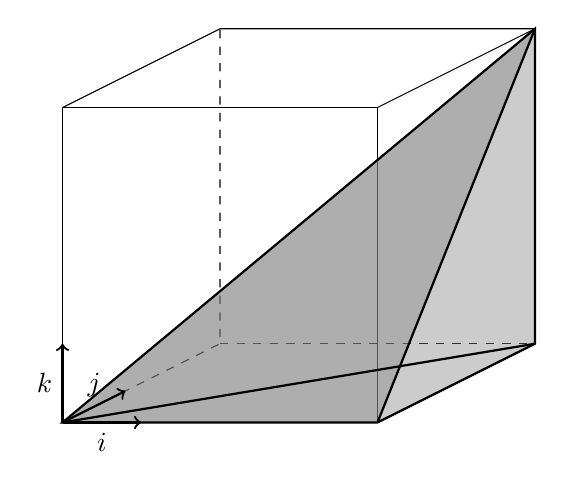
\begin{tikzpicture}
    \draw (0,0) -- (4,0) -- (4,4) -- (0,4) -- cycle;
    \draw (4,0) -- (6,1) -- (6,5) -- (2,5) -- (0,4);
    \draw (4,4) -- (6,5);
    \draw[dashed] (0,0) -- (2,1) -- (2,5);
    \draw[dashed] (2,1) -- (6,1);
    \fill[gray, opacity=.4] (0,0) -- (6,1) -- (6,5) -- cycle;
    \fill[gray, opacity=.4] (0,0) -- (4,0) -- (6,1) -- cycle;
    \fill[gray, opacity=.4] (0,0) -- (4,0) -- (6,5) -- cycle;
    \draw[thick] (0,0) -- (4,0) -- (6,1) -- (6,5) -- cycle;
    \draw[thick] (0,0) -- (6,1);
    \draw[thick] (4,0) -- (6,5);
    \draw[thick,->] (0,0) to node[below]{$i$} (1,0);
    \draw[thick,->] (0,0) to node[above]{$j$} (.8,.4);
    \draw[thick,->] (0,0) to node[left]{$k$} (0,1);
  \end{tikzpicture}
  \caption{Cone obtained by symmetries from Fig.~\ref{fig:symmetries}, and
    requiring $j\le i, \, k\le i, \, k\le j$ contains $16$ far-field
    interactions.}
  \label{fig:cone_sym}
\end{figure}
Finally, all $316$ far-field interactions can be expressed as permutations of
$16$, only. We write them as
\begin{equation}
  \label{eq:permut}
  \Mat{K}_t = \Mat{P}_t \Mat{K}_{p(t)} \Mat{P}_t^\top
\end{equation}
where $p(t):[1,316]\rightarrow[1,16]$ tells us, depending on $t$, which of the
$16$ remaining far-field interactions to use. $\Mat{P}_t$ are the
corresponding permutation matrices.
\begin{note}
  In this document we do not explain how to compute the permutation matrices
  and the function $p(t)$. We assume they are known and we know how to compute
  them. In fact they are part of the precomputation and need to be computed
  only once.
\end{note}

\subsection{Implementation}
\label{sec:m2limplement}
The setup of the $316$ permutation matrices and the SVDs of the $16$ remaining
far-field interactions are part of the precomputation. The computation of a
far-field interaction, given by $t$, consists of $\Mat{f} = \Mat{K}_t\Mat{w}$
(in matrix notation). The vectors $\Mat{f,w} \in \mathbb{R}^{\ell^3}$ contain
the local expansions $(\Mat{f})_m = F_m$ and multipole expansions $(\Mat{w})_n
= W_n$ of a cell-pair whose relative position is given by the translation
vector $t$. However, we do not compute $\Mat{K}_t$ explicitly as in
Eqn.~\eqref{eq:permut} but we use it to compute
\begin{equation}
  \label{eq:newm2l}
  \Mat{f} = \Mat{K}_t \Mat{w} = \Mat{P}_t \Mat{K}_{p(t)} \Mat{P}_t^\top \Mat{w}
\end{equation}
in three steps: (1) we permute multipole expansions $\Mat{w}_t =
\Mat{P}_t^\top \Mat{w}$, (2) we compute permuted local expansions $\Mat{f}_t =
\Mat{K}_{p(t)} \Mat{w}_t$, (3) we permute permuted local expansions $\Mat{f} =
\Mat{P}_t \Mat{f}_t$ (the application of the permutation matrix to a vector
consists of reordering the vector -- no $\unit{flop}$, no matrix-vector
product).

In Algorithm~\ref{alg:unblockedm2l} we present a naive (unblocked) M2L
kernel. It implements the threefold application in a sequential way, hence, we
end up with at most $316$ matrix-vector products.
\begin{algorithm}
  \caption{Unblocked M2L kernel (at most $316$ matrix-vector products)}
  \label{alg:unblockedm2l}
  \begin{algorithmic}[1]
    \Function{unblocked M2L}{target cell $X$ and all far-field
      interactions $I_Y$}   
    \State{retrieve $\Mat{f}$ from $X$}
    \For{all source cells $Y$ in $I_Y$} 
    \State{retrieve $\Mat{w}$ from $Y$ and compute $t$ from cell-pair $(X,Y)$}
    \State{$\Mat{w}_t \gets \Mat{P}_t^\top \Mat{w}$ \Comment{Permute multipole
        expansions}} \label{one} 
    \State{$\Mat{f}_t \gets \Mat{K}_{p(t)} \Mat{w}_t$ \Comment{Compute permuted
        local expansions}} 
    \State{$\Mat{f} \gets \Mat{f} + \Mat{P}_t \Mat{f}_t$ \Comment{Permute
        permuted local expansions}} 
    \EndFor
    \EndFunction
  \end{algorithmic}
\end{algorithm}

In Algorithm~\ref{alg:blockedm2l} we present an improved (blocked)
implementation of the M2L kernel which exploits the symmetries presented in
Sec.~\ref{sec:symmetries}. We introduce $16$ matrices $\Mat{F}_p, \Mat{W}_p
\in \mathbb{R}^{\ell^3 \times n_c}$ (see Line~\ref{permmatWF} in
Algorithm~\ref{alg:blockedm2l}) whose columns store the permuted local and
multipole expansions corresponding to the respective index $p(t)$ they belong
to. The value $n_c=24$ gives the maximal needed number of columns. In other
words, there is no chance that one of the $16$ far-field interactions is
needed more often than $24$ times. Moreover, we need an expansion counter
$\Mat{c} \in \mathbb{N}^{16}$ (see Line~\ref{expcounter}) indicating the
number of columns (expansions) of these matrices. Then, we split the single
loop into three loops. In the first one, we assemble the set of matrices
$\{\Mat{W}_{p(t)}\}$ and at its end $|\Mat{c}| \le 189$ and $\max(\Mat{c}) =
n_c$ is true. In the second one, we perform the $16$ matrix-matrix
products. And in the last one, we increment the local expansions.
\begin{algorithm}
  \caption{Blocked M2L kernel (at most $16$ matrix-matrix products)}
  \label{alg:blockedm2l}
  \begin{algorithmic}[1]
    \Function{blocked M2L}{target cell $X$ and all far-field interactions $I_Y$}
    \State{allocate $\{\Mat{F}_p\}, \{\Mat{W}_p\}$ for $p=1,\dots,16$
      ($\Mat{F}_p, \Mat{W}_p \in \mathbb{R}^{\ell^3\times
        n_e}$)} \label{permmatWF}
    \State{retrieve $\Mat{f}$ from $X$}
    \State{initialize $\Mat{c}=\Mat{0}$
      ($\Mat{c}\in\mathbb{N}^{16}$)} \label{expcounter}  
    \For{all source cells $Y$ in $I_Y$}
    \State{retrieve $\Mat{w}$ from $Y$ and compute $t$ from cell-pair $(X,Y)$}
    \State{column $(\Mat{c})_{p(t)}$ of $\Mat{W}_{p(t)}$ gets $\Mat{P}_t^\top
      \Mat{w}$ \Comment{Permute multipole expansions}}
    \State{increment $(\Mat{c})_{p(t)}$}
    \EndFor
    \For{all $\{\Mat{K}_p\}$}
    \State{$\Mat{F}_p \gets \Mat{K}_p \Mat{W}_p$
      \Comment{Compute permuted local expansions}}
    \EndFor
    \State{reinitialize $\Mat{c}=\Mat{0}$}
    \For{all source cells $Y$ in $I_Y$}
    \State{compute $t$ from cell-pair $(X,Y)$}
    \State{retrieve $\Mat{f}_t$ from column $(\Mat{c})_{p(t)}$ of
      $\Mat{F}_{p(t)}$} 
    \State{increment $(\Mat{c})_{p(t)}$}
    \State{$\Mat{f} \gets \Mat{f} + \Mat{P}_t \Mat{f}_t$
      \Comment{Permute permuted local expansions}} 
    \EndFor
    \EndFunction
  \end{algorithmic}
\end{algorithm}

\begin{table}[htbp]
  \caption{Timing results of the Algorithms~\ref{alg:unblockedm2l} and
    \ref{alg:blockedm2l}: Required time of all M2L kernels for
    $2\cdot10^4$ uniformly distributed particles and $h=5$ 
    on a $\unit[2.26]{GHz}$ Intel Core $2$ Duo without MKL}
  \label{tab:timings_alg1_alg2}
  \centering
    \begin{tabular}{c | r r | c}
      \toprule
      $Acc$ & $\unit[t_1]{[s]}$ & $\unit[t_2]{[s]}$ & $\nicefrac{t_2}{t_1}$ \\  
      \midrule
      3 &  0.4498 &  0.2665 & 0.59 \\
      5 &  2.7170 &  1.7141 & 0.63 \\
      7 & 13.7341 & 11.1773 & 0.81 \\
      \bottomrule
  \end{tabular}
\end{table}


\section{Tensor-product interpolation}
\label{sec:tensorinterpol}
The anterpolation (P2M, M2M) can be understood as the transposed operation of
interpolation (L2L, L2P). In our notation they read as
\begin{equation}
  \label{eq:m2ml2l}
  W_n = \sum_{j=1}^N S_\ell(y_j,\bar y_m) \, w_j, \text{ for }
  n=1,\dots,\ell^3 \qquad \text{and} \qquad
  f_i = \sum_{m=1}^{\ell^3} S_\ell(x_i,\bar x_m) F_m, \text{ for }
  i=1,\dots,M
\end{equation}
and in matrix notation as $\Mat{w}^\prime = \Mat{S}^\top \Mat{w}$ and $\Mat{f}
= \Mat{Sf}^\prime$ if $(^\prime)$ denotes the upper level. In the leaf level
these kernels correspond to P2M (particle-to-moment) and L2P
(local-to-particle) operations. In all other levels they correspond to the M2M
(moment-to-moment) and L2L (local-to-local) operations. Depending on the
level, $M$ and $N$ vary: in the leaf level they denote the number of source
and target particles, in all other levels we have $M=N=\ell^3$. In the
following, we explain the tensor-product interpolation first for the M2M and
L2L kernels and then for the P2M and L2P kernels.


\subsection{M2M and L2L kernels}
\label{sec:m2ml2l}
We assume the uniform case in $\mathbb{R}^3$, i.e., each cell has $8$ child
cells. We address them based on Morton ordering \citep[see][]{Warren1993}
the local position of the child cells is given by their local position $000$
until $111$, if we translate this binary representation we obtain indices from
$0$ to $7$.

\paragraph{Tensor-product}
If we consider the $1$d case in Fig.~\ref{fig:1dm2m} each cell has two child
cells $0$ and $1$ and $\ell$ interpolation points. We set up an interpolation
matrix $\Mat{S}_0, \Mat{S}_1 \in \mathbb{R}^{\ell\times\ell}$ for both of
them. The entries are computed as
\begin{equation}
  \label{eq:interpolmatrixentries}
  (\Mat{S}_i)_{nm} = S_\ell(x_n,\bar x_m)
  \quad \text{with } x_n = \frac{\bar x_n }{2} + \frac{(-1)^{i+1}}{2} \quad
  \text{for } i=1,2 \text{ and } n,m=1,\dots,\ell,
\end{equation}
with the Chebyshev roots, defined as $\bar x_m =
\cos\left(\nicefrac{(2m-1)\pi}{2\ell}\right)$. Finally, the M2M and L2L
kernels consist of applying both matrices $\Mat{S}_0$ and $\Mat{S}_1$ (for
child $0$ and child $1$), respectively.
\begin{figure}[htbp]
  \centering
  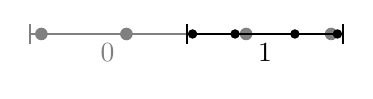
\begin{tikzpicture}[scale=2]
    \draw[gray, thick,|-|] (-1,0) -- (1,0);
    \foreach \i in {-0.92, -0.38,	0.38,	0.92}
    {
      \fill[gray] (\i,0) circle (.04);
      \fill[black] (\i/2+.5,0) circle (.03);
    }
    \draw[thick,|-|] (0,0) -- (1,0);
    \node at (-.5,0) [below,gray] {$0$};
    \node at (.5,0) [below] {$1$};
  \end{tikzpicture}
  \caption{Interpolation points for $\ell=4$ in $\mathbb{R}$: parent cell in
    gray $[-1,1]$ and child cell in black $[0,1]$}
  \label{fig:1dm2m}
\end{figure}

Next, we consider the $\mathbb{R}^3$ case (we think of Fig.~\ref{fig:2dm2m} as
the lower level of child cells): each cell has $8$ child cells and the number
of interpolation points in each cell is $\ell^3$. The most straight forward
(but also the most naive) way of implementing the M2M and L2L kernels would be
to compute $8$ interpolation matrices of size $\ell^3\times\ell^3$.
\begin{figure}[htbp]
  \centering
  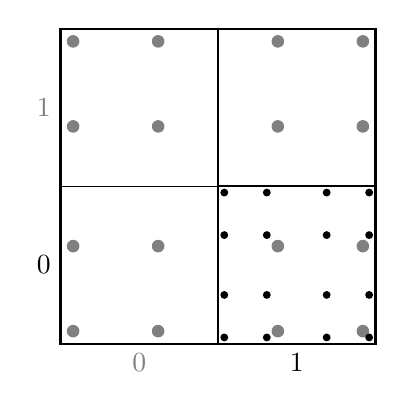
\begin{tikzpicture}[scale=2]
    \draw[thick] (-1,-1) rectangle (1,1);
    \draw[thin] (-1,0) -- (1,0);
    \draw[thin] (0,-1) -- (0,1);
    \draw[thick] (0,-1) rectangle (1,0);

    \foreach \i in {-0.92, -0.38,	0.38,	0.92}
    \foreach \j in {-0.92, -0.38,	0.38,	0.92}
    {
      \fill[gray] (\i,\j) circle (.04);
      \fill[black] (\i/2+.5,\j/2-.5) circle (.025);
    }
    \node at (-.5,-1) [below,gray] {$0$};
    \node at (.5,-1) [below] {$1$};
    \node at (-1,-.5) [left] {$0$};
    \node at (-1,.5) [left,gray] {$1$};
  \end{tikzpicture}
  \caption{Tensor structure of interpolation points for $\ell=4$ in
    $\mathbb{R}^3$ (figure shows the lower level of child cells): parent cell
    in gray $[-1,1] \times [-1,1] \times [-1,1]$ and child cell in black
    $[0,1] \times [-1,0] \times [-1,0]$}
  \label{fig:2dm2m}
\end{figure}
However, by exploiting the tensor-product approach we can construct a more
efficient scheme. We consider the child cell of index $1$ (in binary of Morton
notation $001$) in Fig.~\ref{fig:2dm2m}. The full interpolation matrix
$\Mat{S}_{001}\in\mathbb{R}^{\ell^3\times\ell^3}$ can be defined as a tensor
product (also Kronecker product) and reads as
\begin{equation}
  \label{eq:tensorprod}
  \Mat{S}_{001} = \Mat{S}_0 \times \Mat{S}_0 \times \Mat{S}_1
\end{equation}
Again, we do never compute $\Mat{S}_{001}$ explicitly, but we exploit
properties of the tensor product. In fact, it allows us to reduce the cost
$\mathcal{O}(\ell^6)$ of applying the matrix $\Mat{S}_{001}$ to only
$\mathcal{O}(3\ell^4)$. We use Eqn.~\eqref{eq:tensorprod} to write the M2M
kernel as $\Mat{w}^\prime = \left( \Mat{S}_0 \times \Mat{S}_0 \times \Mat{S}_1
\right)^\top \Mat{w}$ and the L2L kernel as $\Mat{f} = \left( \Mat{S}_0 \times
  \Mat{S}_0 \times \Mat{S}_1 \right) \Mat{f}^\prime$. Recall, we have
constructed also the interpolation points based on the tensor product approach
as $\bar x_m = \bar x_i \times \bar x_j \times \bar x_k$ with $m = k\ell^2 +
j\ell + i$. In the following, we use the indices $i, j, k$ and $i^\prime,
j^\prime, k^\prime$ to address them (indices in $x,y,z$ direction and
$(^\prime)$ denotes the upper level). According to these indices we can
reassemble the vectors $\Mat{w,w}^\prime$ and $\Mat{f,f}^\prime$ as tensors of
size $\ell \times \ell \times \ell$ with the $ijk$-th entry being given by the
$m$-th entry of the vectors, respectively. Finally, by using index notation we
can write the M2M and L2L kernels as
\begin{equation}
  \label{eq:indexm2ml2l}
  (\Mat{w}^\prime)_{i^\prime j^\prime k^\prime} = (\Mat{S}_0)_{kk^\prime}
  (\Mat{S}_0)_{jj^\prime} (\Mat{S}_1)_{ii^\prime} (\Mat{w})_{ijk}
  \quad \text{and} \quad
  (\Mat{f})_{ijk} = (\Mat{S}_0)_{kk^\prime} (\Mat{S}_0)_{jj^\prime}
  (\Mat{S}_1)_{ii^\prime} (\Mat{f}^\prime)_{i^\prime j^\prime k^\prime},
\end{equation}
which can be implemented as three consequent matrix-matrix products followed
by a permutation of the resulting matrices. Each product has a cost of
$\mathcal{O}(\ell^4)$. This operation has to be repeated for each child cell.

\begin{note}
  If we have a look at Fig.~\ref{fig:1dm2m} we recognize the symmetry of the
  interpolation points. Hence, it is also possible to express the matrix $S_1$
  as a permutation of $S_0$. If we follow this idea we could group the $8$
  times $3$ consecutive matrix-matrix products to $8$ larger matrix-matrix
  products. In reality, though, the time required for the M2M and L2L is
  vanishingly small compared to all other kernels. That is why we did not
  further investigate in this optimization.
\end{note}

\subsection{P2M and L2P kernels}
\label{sec:leaflevel}
We cannot extend the tensor-product approach we presented in
Sec.~\ref{sec:m2ml2l} for the P2M and L2P kernels. In the case of M2M and L2L
kernels the evaluation points at both, the child and parent level, form a
uniform (tensor) grid. Here, this is only true for the parent level. The
particles (the equivalent to the child level for the M2M and L2L kernels) are
completely non-uniform.

Nonetheless, we can construct an efficient implementation. Lets stick again
with the $\mathbb{R}$ case, and recall the definition of the interpolation
polynomial in Eqn.~\eqref{eq:interpolation_polynomial}. In order to ease the
explanation we use the notation used in \citep[]{mason2003chebyshev} to rewrite
the interpolation polynomial as
\begin{equation}
  \label{eq:masonnotationinterpol}
  S_\ell(x,\bar x_m) = \frac{2}{\ell} \sum_{\alpha=0}^{\ell-1}{}^\prime
  T_\alpha(x) T_\alpha(\bar x_m)
\end{equation}
where the prime $(^\prime)$ means that the term in the sum for $\alpha=0$ is
divided by $2$. In matrix notation we can write the interpolation polynomial
(hereafter interpolation matrix) $\Mat{S} \in \mathbb{R}^{N\times\ell}$ as an
outer product
\begin{equation}
  \label{eq:interpolouterprod}
  \Mat{S} = \Mat{T} \Mat{\bar T}^\top \quad \text{with }
  \Mat{T} \in \mathbb{R}^{N\times\ell} \text{ and } \Mat{\bar T} \in
  \mathbb{R}^{\ell\times\ell} 
\end{equation}
with the entries
\begin{equation}
  \label{eq:entriesouterprodinterpol}
  (\Mat{T})_{i\alpha} = T_{\alpha-1}(x_i)
  \qquad \text{and} \qquad   
  (\Mat{\bar T})_{m\alpha} = \frac{2\,T_{\alpha-1}(\bar x_m)}{\ell}. 
\end{equation}
The matrix $\Mat{T}$ needs to be computed for each leaf-cell, the matrix
$\Mat{\bar T}$ only once. Hereafter, we will focus only on the $i$-th row
$\Mat{s} = (\Mat{S})_{i:}$ of the interpolation matrix, i.e., we consider the
interpolation of the particle $i$, only. In the outer-product form this
interpolation vector reads as
\begin{equation}
  \label{eq:rowouterprodinterpol}
  \Mat{s}_i = \Mat{t}_i \Mat{\bar T}^\top \quad \text{with } \Mat{t}_i =
  (\Mat{T})_{i:}
\end{equation}

Next, we consider the $\mathbb{R}^3$ case. Since we have separated the
non-uniform part (particles) and the uniform one (interpolation points) we can
apply the tensor-product interpolation on each particle separately. We write
the $i$-th interpolation vector as
\begin{equation}
  \label{eq:rowouterprodinterpoltensor}
  \Mat{s}_i = \left(\Mat{t}_{i_0} \Mat{\bar T}^\top\right) \times
  \left(\Mat{t}_{i_1} \Mat{\bar T}^\top\right) \times \left(\Mat{t}_{i_2}
    \Mat{\bar T}^\top\right)
  = \left(\Mat{t}_{i_0} \times \Mat{t}_{i_1} \times \Mat{t}_{i_2}\right)
  \left(\Mat{T}^\top \times \Mat{T}^\top \times \Mat{T}^\top\right)
\end{equation}
with $x_i = (x_{i_0}, x_{i_1}, x_{i_2})$. Note, for the evaluation of the P2M
and L2P kernels in Eqn.~\eqref{eq:m2ml2l} we do not compute $\Mat{s}_i$
explicitly, but we apply the matrices one after another (analogously to
Eqn.~\eqref{eq:indexm2ml2l} we implement them as matrix-matrix products). The
cost for the P2M and L2P kernels scales like $\mathcal{O}(N\ell^3+\ell^4)$ if
we assume $M\sim N$.
\begin{note}
  The cost of only applying $\Mat{s}_i$ in the 1d case is
  $\mathcal{O}(N\ell)$, however, the assembly of $\Mat{s}_i$ scales like
  $\mathcal{O}(\ell^2)$ (for each particle). We can extend this to the 3d
  case, where the application only of $\Mat{s}_i$ costs
  $\mathcal{O}(N\ell^3)$, however, the assembly costs $\mathcal{O}(\ell^6)$
  floating point operations (for each particle).
\end{note}

\paragraph{Force computation in the L2P kernel} We define the force kernel
$\boldsymbol{K} : \mathbb{R}^3 \times \mathbb{R}^3 \rightarrow \mathbb{R}^3$
as the gradient of the Laplace kernel $K : \mathbb{R}^3 \times \mathbb{R}^3
\rightarrow \mathbb{R}$, i.e.,
\begin{equation}
  \label{eq:force_kernel}
  \boldsymbol{K}(x,y) = \frac{1}{4\pi} \frac{x-y}{|x-y|^2} = -\nabla_x K(x,y).
\end{equation}
Hence, if we want to compute the forces $\boldsymbol{f}_i\in\mathbb{R}^3$
acting on the $i$-th target particle (we use Eqn.~\eqref{eq:fast_summation}
and reformulate it) we have
\begin{equation}
  \label{eq:forcemodel}
  \boldsymbol{f}_i \sim \sum_{m=1}^{\ell^3} \boldsymbol{P}_\ell(x_i, \bar x_m)
  \sum_{n=1}^{\ell^3} K(\bar x_m, \bar y_n) \sum_{j=1}^N S_\ell(y_j, \bar y_n)
  w_j
\end{equation}
with $\boldsymbol{P}_\ell(x, \bar x) = -\nabla_x S_\ell(x, \bar x)$. We notice
that P2M, M2M, M2L and L2L are the same as for the computation as for the
potential, only L2P changes. With the definition of
\begin{equation}
  \label{eq:Pin1d}
  P_\ell(x,\bar x_m) = \frac{2}{\ell} \sum_{\alpha=1}^{\ell-1} \alpha
  U_{\alpha-1}(x) T_\alpha(\bar x_m) \quad \text{for } x\in[-1,1]
\end{equation}
in $1$d and with the definition of $\Mat{s}_i$ in
Eqn.~\eqref{eq:rowouterprodinterpoltensor} we can define also the three
components of the gradient of the $i$-th interpolation vector $\Mat{p}_i$ as
\begin{equation}
  \label{eq:rowouterprodinterpoltensorgradient}
  \Mat{p}_i = 
  \begin{pmatrix}
    (\Mat{u}_{i_0} \times \Mat{t}_{i_1} \times \Mat{t}_{i_2})
    \left(\Mat{\bar U}^\top \times \Mat{\bar T}^\top \times \Mat{\bar
        T}^\top\right)\\ 
    (\Mat{t}_{i_0} \times \Mat{u}_{i_1} \times \Mat{t}_{i_2})
    \left(\Mat{\bar T}^\top \times \Mat{\bar U}^\top \times \Mat{\bar
        T}^\top\right) \\ 
    (\Mat{t}_{i_0} \times \Mat{t}_{i_1} \times \Mat{u}_{i_2})
    \left(\Mat{\bar T}^\top \times \Mat{\bar T}^\top \times \Mat{\bar
        U}^\top\right) 
  \end{pmatrix}
\end{equation}
with $\Mat{u}_{i_d}\in\mathbb{R}^{\ell-1}$ and $\Mat{\bar
  U}\in\mathbb{R}^{\ell\times(\ell-1)}$ and the entries
$(\Mat{u}_{i_d})_{\alpha} = \alpha U_{\alpha-1}(x_{i_d})$ and $(\Mat{\bar
  U})_{m\alpha} = \nicefrac{2T_\alpha(\bar x_m)}{\ell}$. As always,
$\Mat{p}_i$ is never computed explicitly. All components are applied
sequentially and are implemented as matrix-matrix products.


\begin{note}
  In our implementation of the P2M and L2P kernels we did not strictly follow
  the above derivation. But we use the following approach presented by means
  of the L2P kernel, which read as
  \begin{equation*}
    f_i = \sum_{n=1}^{\ell^3} S_\ell(x_i,\bar x_n) F_n \quad \text{for }
    i=1,\dots,N, 
  \end{equation*}
  with
  \begin{equation*}
    S_\ell(x_i, \bar x_n) =
    \Big[\frac{1}{\ell} + \frac{2}{\ell} \sum_{\alpha=1}^{\ell-1} T_\alpha(x_{i_1})
    T_\alpha(\bar x_{n_1})\Big]
    \Big[\frac{1}{\ell} + \frac{2}{\ell} \sum_{\beta=1}^{\ell-1} T_\beta(x_{i_2})
    T_\beta(\bar x_{n_2})\Big]
    \Big[\frac{1}{\ell} + \frac{2}{\ell} \sum_{\gamma=1}^{\ell-1} T_\gamma(x_{i_3})
    T_\gamma(\bar x_{n_3})\Big].
  \end{equation*}
  By reorganizing sums, the above equation can be expressed as
  \begin{equation*}
    f_i = \frac{a+2b_i+4c_i+8d_i}{\ell^3}  \quad \text{for } i=1,\dots,N,
  \end{equation*}
  with
  \begin{align*}
    \label{eq:coeff_outer}
    a = &\sum_{n=1}^{\ell^3} F_n, \\
    b_i = &\sum_{\alpha=1}^{\ell-1} T_\alpha(x_{i_1})
    \sum_{n=1}^{\ell^3} T_\alpha(\bar x_{n_1})F_n + \sum_{\beta=1}^{\ell-1}
    T_\beta(x_{i_2}) \sum_{n=1}^{\ell^3} T_\beta(\bar x_{n_2})F_n +
    \sum_{\gamma=1}^{\ell-1} T_\gamma(x_{i_3}) \sum_{n=1}^{\ell^3} T_\gamma(\bar
    x_{n_3})F_n, \\ 
    c_i  = &\sum_{\alpha=1}^{\ell-1} T_\alpha(x_{i_1}) \sum_{\beta=1}^{\ell-1}
    T_\beta(x_{i_2}) \sum_{n=1}^{\ell^3} T_\alpha(\bar x_{n_1})
    T_\beta(\bar x_{n_2}) F_n + \nonumber\\
    &\sum_{\alpha=1}^{\ell-1} T_\alpha(x_{i_1}) \sum_{\gamma=1}^{\ell-1}
    T_\gamma(x_{i_3}) \sum_{n=1}^{\ell^3} T_\alpha(\bar x_{n_1}) T_\gamma(\bar
    x_{n_3}) F_n + \nonumber\\ 
    &\sum_{\beta=1}^{\ell-1} T_\beta(x_{i_2}) \sum_{\gamma=1}^{\ell-1}
    T_\gamma(x_{i_3}) \sum_{n=1}^{\ell^3} T_\beta(\bar x_{n_2}) T_\gamma(\bar
    x_{n_3}) F_n, \\
    d_i = & \sum_{\alpha=1}^{\ell-1} T_\alpha(x_{i_1}) \sum_{\beta=1}^{\ell-1}
    T_\beta(x_{i_2}) \sum_{\gamma=1}^{\ell-1} T_\gamma(x_{i_3})
    \sum_{n=1}^{\ell^3}  T_\alpha(\bar x_{n_1})  T_\beta(\bar x_{n_2})
    T_\gamma(\bar x_{n_3}) F_n
  \end{align*}
  The overall complexity does not change.
\end{note}



%The L2P operation read as
%\begin{equation}
%  \label{eq:l2p_formula}
%  f_i = \sum_{n=1}^{\ell^3} S_\ell(x_i,\bar x_n) F_n \quad \text{for } i=1,\dots,N,
%\end{equation}
%with
%\begin{equation}
%  \label{eq:interpol_expre}
%  S_\ell(x_i, \bar x_n) =
%  \Big[\frac{1}{\ell} + \frac{2}{\ell} \sum_{\alpha=1}^{\ell-1} T_\alpha(x_{i_1})
%  T_\alpha(\bar x_{n_1})\Big]
%  \Big[\frac{1}{\ell} + \frac{2}{\ell} \sum_{\beta=1}^{\ell-1} T_\beta(x_{i_2})
%  T_\beta(\bar x_{n_2})\Big]
%  \Big[\frac{1}{\ell} + \frac{2}{\ell} \sum_{\gamma=1}^{\ell-1} T_\gamma(x_{i_3})
%  T_\gamma(\bar x_{n_3})\Big].
%\end{equation}
%By reorganizing sums, Eqn.~\eqref{eq:interpol_expre} can be expressed in an
%outer-product form as
%\begin{equation}
%  \label{eq:outer_prod}
%  f_i = \frac{a+2b_i+4c_i+8d_i}{\ell^3}  \quad \text{for } i=1,\dots,N,
%\end{equation}
%with
%\begin{align}
%  \label{eq:coeff_outer}
%  a = &\sum_{n=1}^{\ell^3} F_n, \\
%  b_i = &\sum_{\alpha=1}^{\ell-1} T_\alpha(x_{i_1})
%  \sum_{n=1}^{\ell^3} T_\alpha(\bar x_{n_1})F_n + \sum_{\beta=1}^{\ell-1}
%  T_\beta(x_{i_2}) \sum_{n=1}^{\ell^3} T_\beta(\bar x_{n_2})F_n +
%  \sum_{\gamma=1}^{\ell-1} T_\gamma(x_{i_3}) \sum_{n=1}^{\ell^3} T_\gamma(\bar
%  x_{n_3})F_n, \\ 
%  c_i  = &\sum_{\alpha=1}^{\ell-1} T_\alpha(x_{i_1}) \sum_{\beta=1}^{\ell-1}
%  T_\beta(x_{i_2}) \sum_{n=1}^{\ell^3} T_\alpha(\bar x_{n_1})
%   T_\beta(\bar x_{n_2}) F_n + \nonumber\\
%  &\sum_{\alpha=1}^{\ell-1} T_\alpha(x_{i_1}) \sum_{\gamma=1}^{\ell-1}
%  T_\gamma(x_{i_3}) \sum_{n=1}^{\ell^3} T_\alpha(\bar x_{n_1}) T_\gamma(\bar
%  x_{n_3}) F_n + \nonumber\\ 
%  &\sum_{\beta=1}^{\ell-1} T_\beta(x_{i_2}) \sum_{\gamma=1}^{\ell-1}
%  T_\gamma(x_{i_3}) \sum_{n=1}^{\ell^3} T_\beta(\bar x_{n_2}) T_\gamma(\bar
%  x_{n_3}) F_n, \\
%  d_i = & \sum_{\alpha=1}^{\ell-1} T_\alpha(x_{i_1}) \sum_{\beta=1}^{\ell-1}
%  T_\beta(x_{i_2}) \sum_{\gamma=1}^{\ell-1} T_\gamma(x_{i_3})
%  \sum_{n=1}^{\ell^3}  T_\alpha(\bar x_{n_1})  T_\beta(\bar x_{n_2})
%  T_\gamma(\bar x_{n_3}) F_n,
%\end{align}
%where the indices in $x_i = (x_{i_1}, x_{i_2}, x_{i_3})$ and $\bar x_n = (\bar
%x_{n_1}, \bar x_{n_2}, \bar x_{n_3})$ address the individual coordinates of
%the respective points in $\mathbb{R}^3$. In matrix-notation these operators
%read as
%\begin{align}
%  \label{eq:mat_coeff_outer}
%  b_i = &(\Mat{x}_i \otimes \i \otimes \i) (1 \otimes 1 \otimes \Mat{T})^\top
%  \Mat{F} + (\i \otimes \Mat{y}_i \otimes \i) (1 \otimes \Mat{T} \otimes
%  1)^\top \Mat{F} + (\i \otimes \i \otimes \Mat{z}_i)
%  (\Mat{T} \otimes 1 \otimes 1)^\top \Mat{F}, \\
%  c_i = &(\Mat{x}_i \otimes \Mat{y}_i \otimes \i) (1 \otimes \Mat{T} \otimes
%  \Mat{T})^\top \Mat{F} + (\Mat{x}_i \otimes \Mat{y}_i \otimes \i) (1 \otimes
%  \Mat{T} \otimes \Mat{T})^\top \Mat{F} + (\i \otimes \Mat{y}_i \otimes
%  \Mat{z}_i) (\Mat{T} \otimes \Mat{T} \otimes 1)^\top \Mat{F}, \\
%  d_i = &(\Mat{x}_i \otimes \Mat{y}_i \otimes \Mat{z}_i) (\Mat{T \otimes T
%    \otimes T})^\top \Mat{F}.
%\end{align}
%with the matrices $(\Mat{T})_{\alpha n} = T_\alpha(\bar x_n)$ and $(1)_{\alpha
%  n} = 1$ and the vectors $(\Mat{x}_i)_\alpha = T_\alpha(x_{i_1})$ and
%$(\i)_\alpha = 1$, $(\Mat{y}_i)_\alpha = T_\alpha(x_{i_2})$ and
%$(\Mat{z}_i)_\alpha = T_\alpha(x_{i_3})$ for $\alpha=1,\dots,\ell-1$ and
%$n=1,\dots,\ell$.



%%\begin{align}
%%  S&= \frac{1}{\ell^3} \left[1 + 2 \left(\sum_{n=1}^{\ell-1} T_n(x_{i_1})
%%      T_n(\bar x_{m_1}) + \sum_{n=1}^{\ell-1} T_n(x_{i_2}) T_n(\bar x_{m_2}) +
%%      \sum_{n=1}^{\ell-1} T_n(x_{i_3}) T_n(\bar x_{m_3})\right) \right.\nonumber\\
%%  &\qquad+ 4 \left(\sum_{n=1}^{\ell-1} T_n(x_{i_1}) T_n(\bar x_{m_1})
%%      \sum_{n=1}^{\ell-1} T_n(x_{i_2}) T_n(\bar x_{m_2}) \right.\nonumber\\
%%    &\qquad\quad\;\;+ \sum_{n=1}^{\ell-1} T_n(x_{i_1}) T_n(\bar x_{m_1})
%%    \sum_{n=1}^{\ell-1} T_n(x_{i_3}) T_n(\bar x_{m_3})\nonumber\\
%%    &\qquad\quad\;\;\left. + \sum_{n=1}^{\ell-1} T_n(x_{i_2}) T_n(\bar x_{m_2})
%%      \sum_{n=1}^{\ell-1} T_n(x_{i_3}) T_n(\bar x_{m_3}) \right) \nonumber\\
%%    &\qquad\left.+ 8 \sum_{n=1}^{\ell-1} T_n(x_{i_1})
%%      T_n(\bar x_{m_1}) \sum_{n=1}^{\ell-1} T_n(x_{i_2}) T_n(\bar x_{m_2})
%%      \sum_{n=1}^{\ell-1} T_n(x_{i_3}) T_n(\bar x_{m_3})\right]
%%\end{align}
%%where $m$ and $i$ are multi-indices.
%
%\subsection{Counting floating point operations}
%\label{sec:flop_counting}
%
%
%
%%\paragraph{P2M, M2M, L2L and L2P} The cost for evaluating Chebyshev
%%polynomials $T_\ell(x)$ in terms of number of floating point operations (by
%%using the recursive definition $T_n(x) = 2xT_{n-1}-T_{n-1}, \, T_0(x)=1, \,
%%T_1(x)=x$ and $U_n(x) = 2xU_{n-1}-U_{n-1}, \, U_0(x)=1, \, U_1(x)=2x$ and
%%reusing intermediate results) is
%%\begin{equation}
%%  \label{eq:flop_cheb}
%%  \flop(T_n) = 3(n-1) \qquad \text{and} \qquad \flop(U_n) = 3(n-1)+1
%%\end{equation}
%%and the cost for evaluating $S_\ell(x,\bar x)$ and $P_\ell(x,\bar x) =
%%\nabla_x S(x,\bar x)$ in $\mathbb{R}^1$ is
%%\begin{align}
%%  \label{eq:flop_interpolator}
%%  \flop(S_\ell) &= 4 + 2\flop(T_{\ell-1}) + 2(\ell-1) = 8\ell-10,\\
%%  \flop(P_\ell) &= 2 + \flop(U_{\ell-2}) + \flop(T_{\ell-1}) + 3(\ell-1) =
%%  9\ell-15
%%\end{align}
%%which is also the cost for computing an entry of the P2M, M2M, L2L and L2P
%%operators. Hence, the computation of the matrices
%%$\Mat{S}\in\mathbb{R}^{N\times\ell^3}$ and
%%$\Mat{P}\in\mathbb{R}^{3N\times\ell^3}$, where $N$ denotes the number of
%%particles and $\ell$ the interpolation order, has a cost of
%%\begin{align}
%%  \label{eq:flop_S_matrix}
%%  \flop(\Mat{S}) &= N \ell^3 \left(3\flop(S_\ell) + 2\right) =
%%  N\ell^3(24\ell-28), \\
%%  \flop(\Mat{P}) &= N \ell^3 \left(3\flop(S_\ell)+3\flop(P_\ell) + 6\right) = 3N\ell^3(17\ell-23),
%%\end{align}
%%and finally the overall cost for performing the matrix-vector products
%%$\Mat{Sw}$ and $\Mat{Pw}$ is
%%\begin{align}
%%  \label{eq:flop_mat_vec}
%%  \flop(\Mat{Sw}) &= \flop(\Mat{S}) + N(2\ell^3-1) =
%%  N\left(\ell^3(24\ell-26)-1\right), \\
%%  \flop(\Mat{Pw}) &= \flop(\Mat{P}) + 3N(2\ell^3-1) =
%%  3N\left(\ell^3(17\ell-21)-1\right).
%%\end{align}
%%Recall, in the case of the L2L and L2P operator, ie.~$\Mat{p}+\Mat{Sw}
%%\rightarrow \Mat{p}$ and $\Mat{f}+\Mat{Pw} \rightarrow \Mat{f}$ another $N$,
%%respectively $3N$, floating point operations have to be added to the flop
%%count.
%
%%\paragraph{M2L} The cost of performing an SVD of
%%$\Mat{K}\in\mathbb{R}^{\ell^3\times\ell^3}$ sums up to $\flop(\Mat{U\Sigma
%%  V}^\top) = 21(\ell^3)^3$ (see \citet{golubVanLoan:96}), and has to be done
%%$16$ times, hence $\flop(\Mat{U\Sigma V}^\top) = 336 \, \ell^6$. To be
%%continued \dots
%
%
%
%%\begin{table}[htbp]
%%  \centering
%%    \begin{tabular}{c | c c | c c | c c | c c}
%%    \toprule
%%    $\#$ Treads &
%%    \multicolumn{2}{c|}{P2M} & \multicolumn{2}{c|}{M2M} &
%%    \multicolumn{2}{c|}{L2L} & \multicolumn{2}{c}{L2P} \\
%%    \midrule
%%    $1$ & 0.370&0.160 & 0.024&0.042 & 0.024&0.046 & 1.079&0.325 \\
%%    $2$ & 0.193&0.091 & 0.012&0.022 & 0.012&0.021 & 0.544&0.168 \\
%%    $4$ & 0.096&0.045 & 0.006&0.011 & 0.006&0.011 & 0.287&0.089 \\
%%    $8$ & 0.080&0.045 & 0.120&0.018 & 0.003&0.005 & 0.154&0.056 \\
%%    \midrule
%%    $1$& 3.323&0.526 & 0.262&0.150  & 0.268&0.146 & 7.074&1.041 \\
%%    $2$& 1.645&0.270 & 0.129&0.077  & 0.129&0.073 & 3.544&0.524 \\
%%    $4$& 0.824&0.135 & 0.065&0.038  & 0.065&0.037 & 1.789&0.272 \\
%%    $8$& 0.453&0.114 & 0.036&0.044  & 0.036&0.018 & 0.906&0.142 \\
%%    \midrule
%%    $1$&11.535&1.251 & 3.244&0.265  & 3.491&0.265 & 30.537&2.421 \\
%%    $2$&5.750 &0.637 & 1.472&0.137  & 1.554&0.134 & 15.326&1.216 \\
%%    $4$&2.863 &0.322 & 0.714&0.070  & 0.746&0.068 & 7.655 &0.618 \\
%%    $8$&1.530 &0.227 & 0.392&0.035  & 0.403&0.034 & 3.840 &0.317 \\
%%    \bottomrule
%%  \end{tabular}
%%  \caption{Comparison of timings for \textsf{SymCheb} before and after
%%    optimization (uniform particle distribution)}
%%  \label{tab:comp_unif_optim}
%%\end{table}
%
%%\begin{table}[htbp]
%%  \centering
%%    \begin{tabular}{c | c c | c c | c c | c c}
%%    \toprule
%%    $\#$ Treads &
%%    \multicolumn{2}{c|}{P2M} & \multicolumn{2}{c|}{M2M} &
%%    \multicolumn{2}{c|}{L2L} & \multicolumn{2}{c}{L2P} \\
%%    \midrule
%%    $1$ & 0.385&0.401 & 0.073&0.147 & 0.070&0.145 & 1.132&0.554\\
%%    $2$ & 0.209&0.221 & 0.043&0.081 & 0.042&0.077 & 0.586&0.283\\
%%    $4$ & 0.107&0.114 & 0.022&0.040 & 0.021&0.039 & 0.294&0.140\\
%%    $8$ & 0.111&0.105 & 0.012&0.021 & 0.011&0.023 & 0.148&0.297\\
%%    \midrule
%%    $1$& 3.401&1.034  & 0.933&0.535 & 0.909&0.520 & 7.137&1.743\\
%%    $2$& 1.694&0.537  & 0.452&0.273 & 0.451&0.260 & 3.593&0.884\\
%%    $4$& 0.843&0.274  & 0.228&0.137 & 0.227&0.129 & 1.824&0.438\\
%%    $8$& 0.455&0.198  & 0.124&0.068 & 0.125&0.065 & 0.870&0.218\\
%%    \midrule
%%    $1$&11.439&1.033  & 1.409&0.135 & 1.480&0.132 &30.544&2.147\\
%%    $2$&5.671 &0.525  & 0.647&0.069 & 0.660&0.067 &14.954&1.086\\
%%    $4$&2.855 &0.262  & 0.325&0.035 & 0.338&0.034 &13.403&1.641\\
%%    $8$&1.441 &0.183  & 0.172&0.017 & 0.174&0.017 & 9.739&2.902\\
%%    \bottomrule
%%  \end{tabular}
%%  \caption{Timings $\unit[t]{[s]}$ for particle distribution on a sphere for
%%    \textsf{SymCheb} after optimization}
%%  \label{tab:comp_spher_optim}
%%\end{table}



\section{Splitting the outer product in the interpolation polynomial}
\label{sec:splitouter}

We introduce the notation of the interpolation polynomial based on the
notation from \cite{mason2003chebyshev}, the interpolation of a function
$p(x)$ reads as
\begin{equation}
  \label{eq:masondef}
  p(x) \sim \sum_{n=0}^{\ell-1} \gamma_n c_n T_n(x)
\end{equation}
with $\gamma_0=1$ and $\gamma_n=2$ for $n\ge1$ and with
\begin{equation}
  \label{eq:chebcoeff}
  c_n = \frac{1}{\ell} \sum_{k=1}^\ell p(\bar x_n) T_k(\bar x_n)
\end{equation}
After inserting Eqn.~(\ref{eq:chebcoeff}) into Eqn.~(\ref{eq:masondef}) we end
up with
\begin{equation}
  \label{eq:outprod}
  p(x) \sim \frac{1}{\ell} \sum_{n=1}^\ell p(\bar x_n) \sum_{k=0}^{\ell-1}
  \gamma_k T_k(\bar x_n) T_k(x)
\end{equation}
In the discrete case, i.e., we have $N$ scattered points $\{x_i\}_{i=1}^N
\subset [-1,1]$, we write Eqn.~\eqref{eq:outprod} in matrix notation as
\begin{equation}
  \label{eq:interpolmatnot}
  \Mat{p} \sim \Mat{T}_x \Mat{\bar T}_x^\top \Mat{\bar p}
\end{equation}
with the matrices $\Mat{T}_x \in \mathbb{R}^{N\times\ell}$ with
$(\Mat{T}_x)_{ik} = T_{k-1}(x_i)$ and $\Mat{\bar T}_x \in
\mathbb{R}^{\ell\times\ell}$ with $(\Mat{\bar T}_x)_{nk} =
\nicefrac{\gamma_{k-1}}{\ell} \, T_{k-1}(\bar x_n)$. Using this notation the
interpolated kernel function $K(x,y)$ reads as
\begin{equation}
  \label{eq:kinterpolmatnot}
  \Mat{K} \sim \Mat{T}_x \Mat{\bar T}_x^\top \Mat{\bar K} (\Mat{T}_y
  \Mat{\bar T}_y^\top)^\top
\end{equation}
With the low-rank representation $\Mat{\bar K} \sim \Mat{UV}^T$ we compute
$\Mat{\bar U} = \Mat{\bar T}_x^\top \Mat{U}$ and $\Mat{\bar V} = \Mat{\bar
  T}_y^\top \Mat{V}$ and write Eqn.~\eqref{eq:kinterpolmatnot} as
\begin{equation}
  \label{eq:kinterpolmatnot1}
  \Mat{K} \sim \Mat{T}_x \Mat{\bar U} \Mat{\bar V}^\top \Mat{T}_y^\top
\end{equation}

\paragraph{Can we still use symmetries?} Recall the approach we proposed in
Sec.~\ref{sec:m2l}. It exploits the symmetries in the arrangement of the
far-field interactions. As we see from Eqn.~\eqref{eq:permut} in that case we
need permutation matrices $\Mat{P}_t$ for the $t$-th far-field interaction and
Eqn.~\eqref{eq:kinterpolmatnot} becomes
\begin{equation}
  \label{eq:symsplit}
  \Mat{K}_t \sim \Mat{T}_x \Mat{\bar T}_x^\top (\Mat{P}_t \Mat{\bar K}_{p(t)}
  \Mat{P}_t^\top) (\Mat{T}_y \Mat{\bar T}_y^\top)^\top.
\end{equation}
With $\Mat{\bar K}_{p(t)} \sim \Mat{U}_{p(t)} \Mat{V}_{p(t)}^\top$ the
matrices in the outer product in Eqn.~\eqref{eq:kinterpolmatnot1} become
$\Mat{\bar U}_t = \Mat{\bar T}_x^\top \Mat{P}_t \Mat{U}_{p(t)}$ and $\Mat{\bar
  V}_t = \Mat{\bar T}_y^\top \Mat{P}_t \Mat{V}_{p(t)}$. Thus, it is not
possible anymore to use the fact that due to symmetries we can express all
$316$ far-field interactions by permutations of $16$ only.





%%% Local Variables: 
%%% mode: latex
%%% TeX-master: "main"
%%% End: 



% references with bibtex
\bibliographystyle{plainnat}
%bibliography{string_abbrev,mathematics,ownbooks,fastmethods,computing,biblio.bib}
\bibliography{cheb.bib}

\end{document}



%%% Local Variables: 
%%% mode: latex
%%% TeX-master: t
%%% End: 
